\documentclass[12pt]{article}

\usepackage{amsmath}    % need for sub-equations
\usepackage{graphicx}   % need for figures
\usepackage{verbatim}   % useful for program listings
\usepackage{color}      % use if color is used in text
\usepackage{subfigure}  % use for side-by-side figures
\usepackage{hyperref}   % use for hypertext links, including those to external documents and URLs
% \usepackage[showframe]{geometry} % remove gay indentation 
% \usepackage{gensymb} % allows me to use fancy symbols in-text


\usepackage{graphicx} % use for images
\graphicspath{ {./images/} } % set path used for images

\setlength{\baselineskip}{16.0pt}    % 16 pt usual spacing between lines

\setlength{\parskip}{3pt plus 2pt}
\setlength{\parindent}{20pt}    
\setlength{\oddsidemargin}{0.5cm}
\setlength{\evensidemargin}{0.5cm}
\setlength{\marginparsep}{0.75cm}
\setlength{\marginparwidth}{2.5cm}s
\setlength{\marginparpush}{1.0cm}
\setlength{\textwidth}{150mm}


 \begin{comment}
    \pagestyle{empty} % doesn't count for page numbers
 \end{comment}
        
        
\begin{document}
        
        \title{A Mathematical Exploration of the Hover Slam Manuever}
        \date{25.10.2018}
        \author{Candiate code: hjk123}            \begin{titlepage}
                \begin{center}
                  % \small{Mathematics SL, IA:} \\
                \Huge{A Mathematical Exploration of the \\ Decay of Caffine}
                \break
                {\large A Mathematics Internal Assessment}
                \break                    %\small{Written by Johan-Petter R. Dragic}
                 % \date{06.11.2018}
                    
        
                    % ADD BREAK HERE
                \vspace{12mm}
                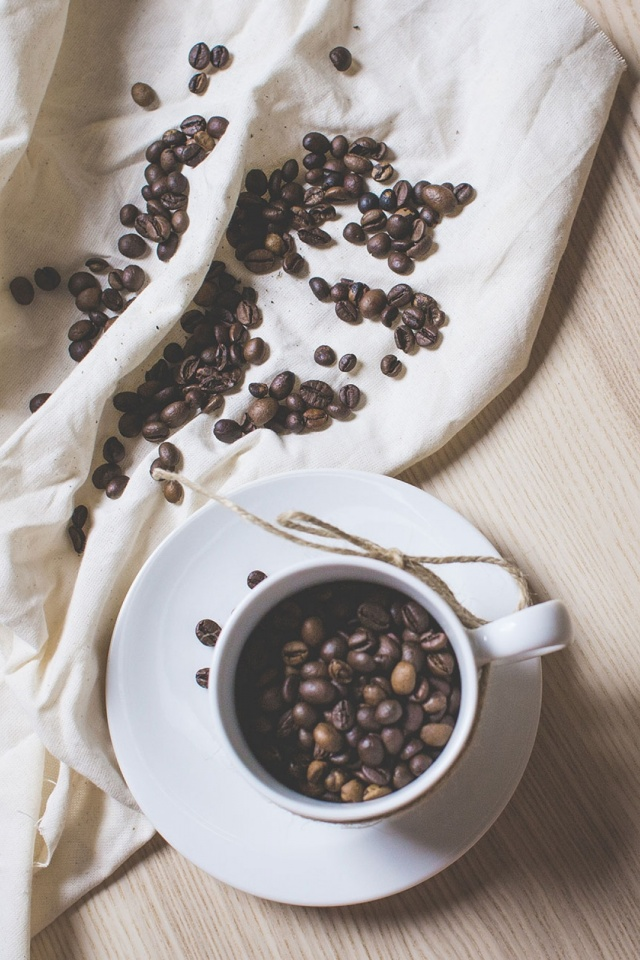
\includegraphics[scale=0.38]{coffee1.jpg}
                % source pic:http://www.mobileswall.com/wallpaper/coffee-beans-in-a-coffee-cup-free/            
    
            \end{center}
                    \end{titlepage}
        
            \tableofcontents
            \thispagestyle{empty}
            \addtocounter{page}{-1}
            


            %%%%%%%%%%%%%%%%%%%%%%%%%%%%%    START OF DOCUMENT    %%%%%%%%%%%%%%%%%%%%%%%%%%%%%%%%%%%%%%%% 
            \newpage
            \section{Introduction} % and personal engagement
            \paragraph
                Coffee has become an integral part of many lives, including mine. It's what wakes you up in the morning and sustains your energy-levels throughout the day. The leading chemical stimulant in coffee is called caffeine and it's classified as a "Psychoactive drug", meaning that it alters the chemical processes that goes on in your brain. The main effect of caffeine is to alter the brain's perception of when it's tired, and is the reason why I and many others admire this mild drug. And since the world average amount of sleep lies bellow the hourly optimum, it is no wonder why caffeine consumed to such extents as it is today.
                \\
                Caffeine is usually consumed through mediums such as tea, coffee and energy drinks (Redbull etc.) and due to the ease of consumption  
\end{document}

